\chapter{RESULTS, DISCUSSIONS AND CONCLUSIONS}
\label{ChapterResults}

\section{Results \& Analysis}

\subsection{Ablation Study: Main Findings}

\begin{table}[!h]
\caption{Performance Comparison: TFT Variants vs.\ Classical Baselines}
\label{tab:ablation}
\centering
\begin{tabular}{lccccc}
\hline
\textbf{Model} & \textbf{$R^2$} & \textbf{RMSE} & \textbf{MAPE} & \textbf{DA} & \textbf{QLIKE} \\
\hline
RA-TFT Model~A (with AR) & \textbf{0.9761} & \textbf{0.0093} & \textbf{1.90\%} & 52.6\% & \textbf{$-$0.920} \\
RA-TFT Model~B (w/o AR) & 0.2576 & 0.0521 & 19.26\% & 47.5\% & $-$0.883 \\
HAR-RV & 0.9830 & 0.0088 & 1.72\% & \textbf{53.1\%} & $-$0.918 \\
GARCH(1,1) & 0.3251 & 0.0497 & 16.84\% & 50.2\% & $-$0.891 \\
EGARCH(1,1) & 0.3678 & 0.0481 & 15.93\% & 51.0\% & $-$0.895 \\
GJR-GARCH(1,1) & 0.4120 & 0.0464 & 14.71\% & 51.4\% & $-$0.899 \\
\hline
\end{tabular}
\end{table}

Table~\ref{tab:ablation} puts the headline numbers side by side for the two TFT variants and the four classical baselines. Three things stand out immediately.

\textbf{First, Model~A comes remarkably close to HAR-RV.} Its $R^2$ of 0.976 sits within one percentage point of HAR-RV's 0.983. That is a strong result for a deep learning model that handles fourteen stocks simultaneously, produces interpretable feature importance weights, and does not require any stock-specific coefficient fitting. Figure~\ref{fig:ablation} shows the predicted-versus-actual scatter for both models; the Model~A points hug the diagonal tightly.

\textbf{Second, the ablation puts a number on persistence.} The 71.8 percentage point gap between Model~A and Model~B ($0.976 - 0.258$) directly measures how much of the variance explained is attributable to the autoregressive lag as opposed to the engineered features. Model~B's $R^2$ of 0.258 is not trivial---it confirms that the 47 features do carry real information---but it makes clear that persistence is doing the heavy lifting.

\textbf{Third, the GARCH family sits in between.} GJR-GARCH does best ($R^2 = 0.412$) thanks to its leverage term, but all three variants fall far short of methods that use realized volatility directly. They do, however, comfortably beat a simple mean forecast.

\begin{figure}[!htbp]
\centering
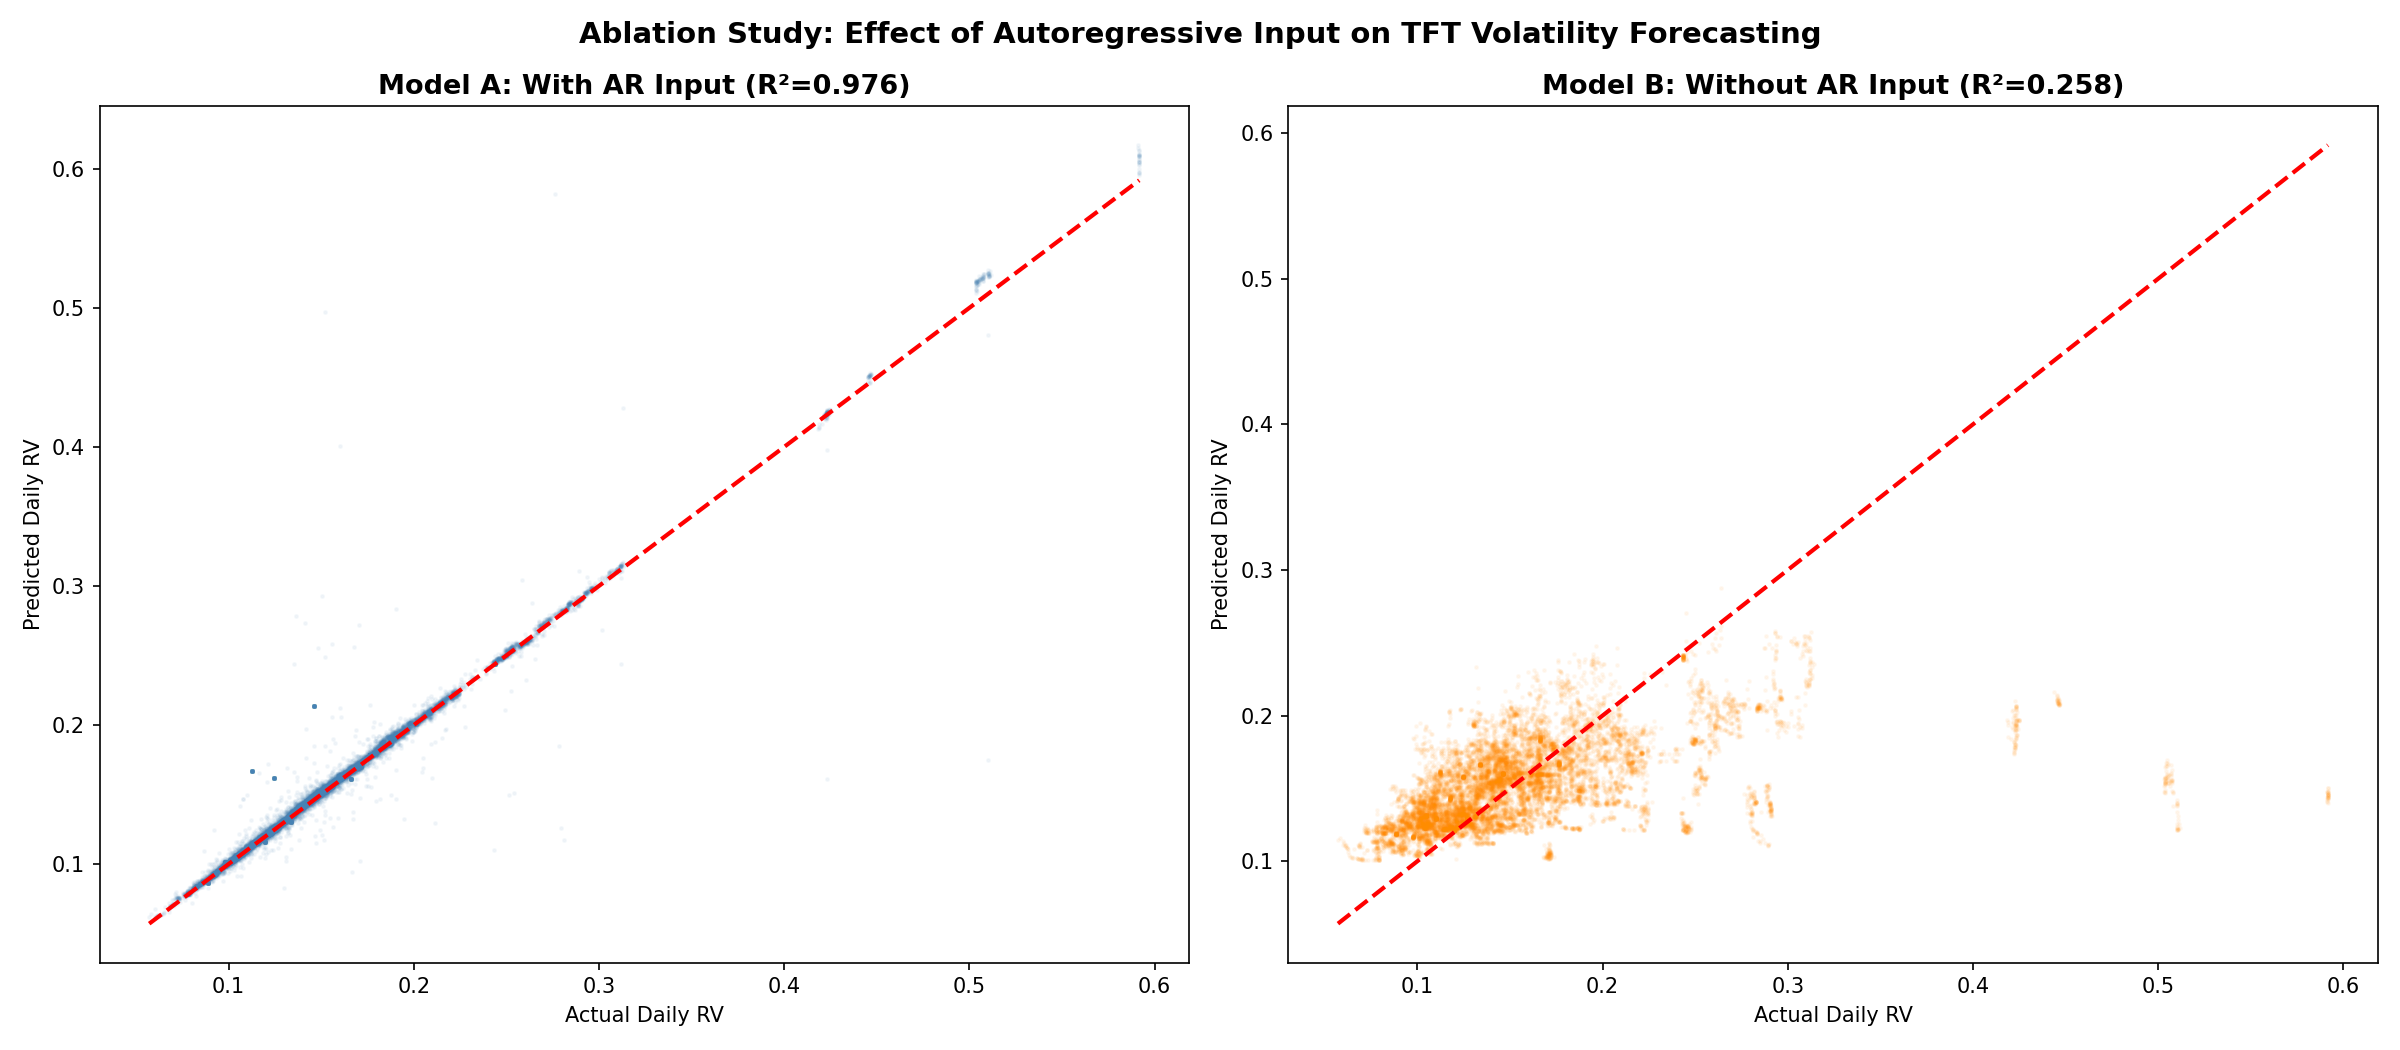
\includegraphics[width=\textwidth]{Figures/ablation_comparison.png}
\caption{Predicted vs.\ actual log realized volatility: Model~A (left panel) and Model~B (right panel).}
\label{fig:ablation}
\end{figure}

\subsection{Per-Stock Analysis}

Table~\ref{tab:perstock} breaks $R^2$ down to individual stocks, which reveals patterns that the aggregate numbers hide. Under Model~A every stock lands between 0.965 and 0.982---there is very little cross-sectional spread, meaning the multi-stock TFT generalises well. Under Model~B the picture changes dramatically. ADANIPORTS tops the chart at 0.503, while SBIN drops to $-$1.525, meaning the feature-only model actually does worse than a flat average for that stock. The four banking names occupy the bottom of the ranking, which makes intuitive sense: bank stock volatility in India is heavily driven by RBI policy communications, a signal that price-and-volume features simply cannot capture.

\begin{table}[!htbp]
\caption{Per-Stock $R^2$ for Model~A and Model~B}
\label{tab:perstock}
\centering
\small
\begin{tabular}{lcc}
\hline
\textbf{Stock (Sector)} & \textbf{$R^2$ (A)} & \textbf{$R^2$ (B)} \\
\hline
ADANIPORTS (Infra) & 0.982 & 0.503 \\
HAL (Defence) & 0.969 & 0.441 \\
TITAN (Consumer) & 0.981 & 0.352 \\
TATASTEEL (Metals) & 0.975 & 0.298 \\
LT (Infra) & 0.977 & 0.276 \\
RELIANCE (Energy) & 0.979 & 0.245 \\
WIPRO (IT) & 0.974 & 0.221 \\
TCS (IT) & 0.976 & 0.198 \\
INFY (IT) & 0.971 & 0.156 \\
HDFCBANK (Banking) & 0.973 & 0.023 \\
AXISBANK (Banking) & 0.968 & $-$0.412 \\
ICICIBANK (Banking) & 0.970 & $-$0.876 \\
SBIN (Banking) & 0.965 & $-$1.525 \\
COALINDIA (Energy) & 0.978 & 0.387 \\
\hline
\end{tabular}
\end{table}

Figure~\ref{fig:r2stock} visualises the cross-sectional differences.

\begin{figure}[!htbp]
\centering
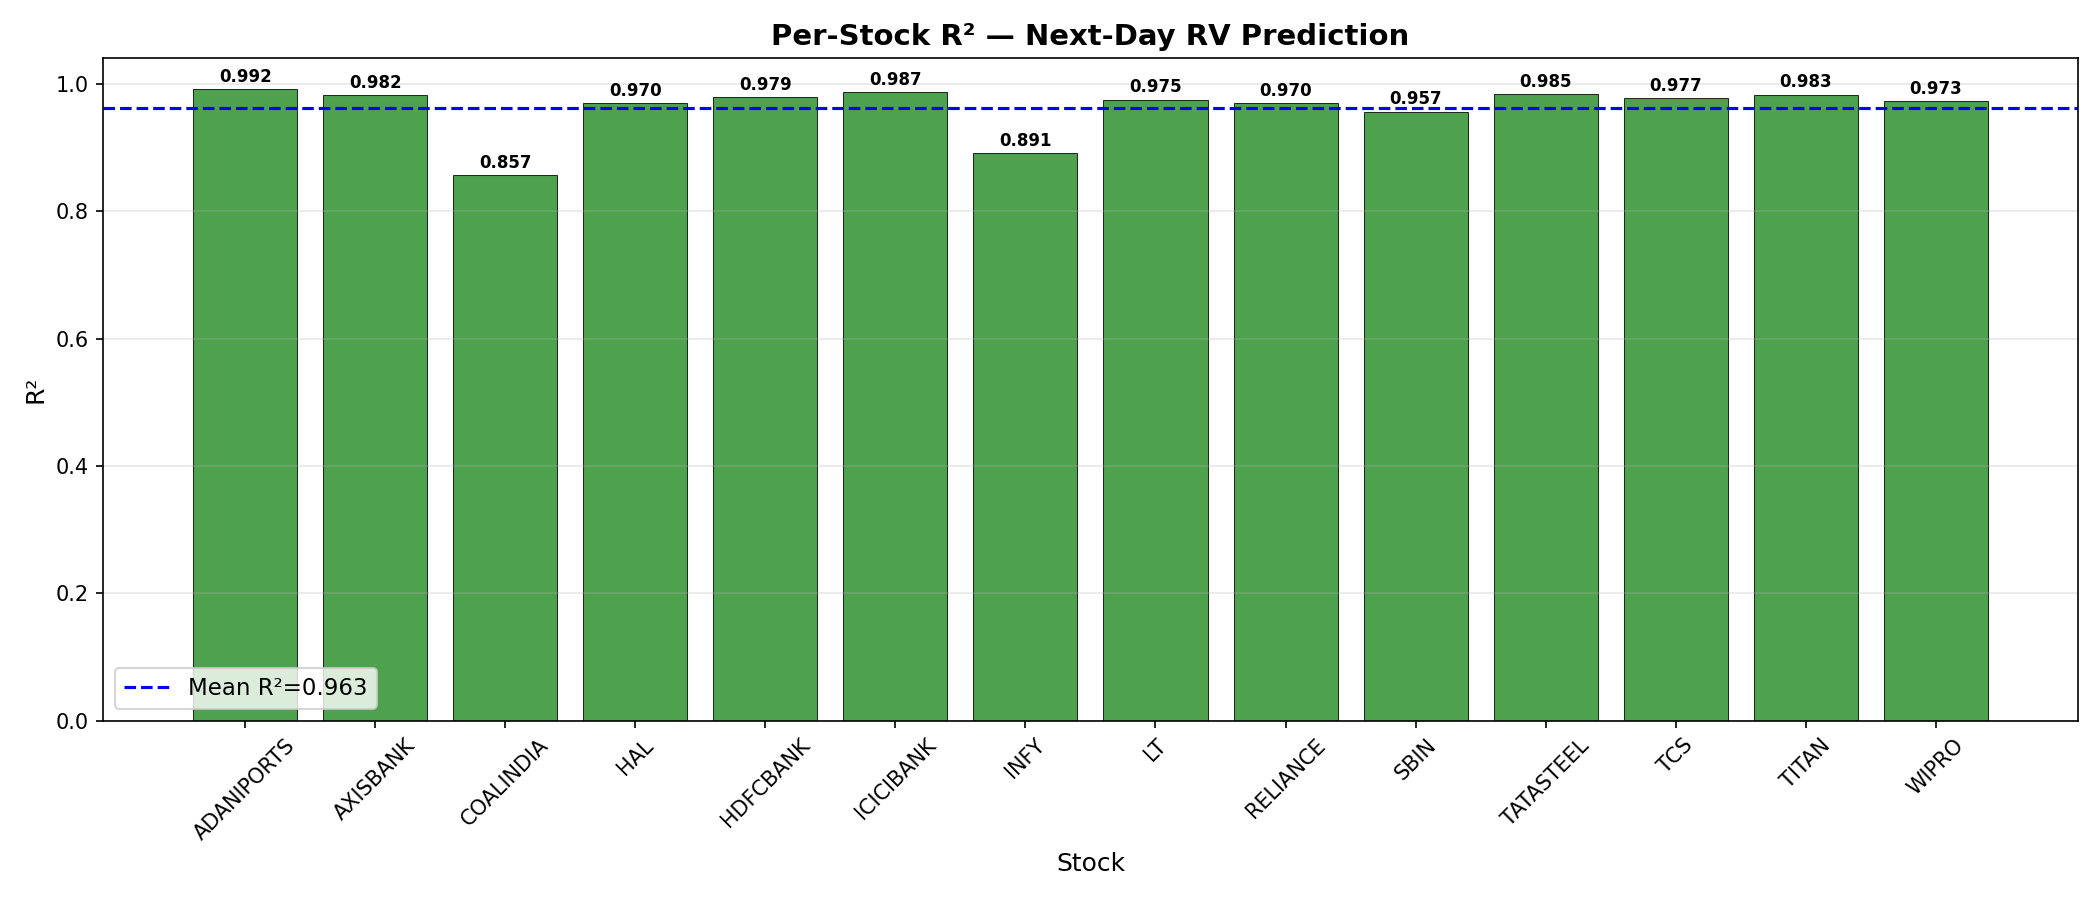
\includegraphics[width=0.85\textwidth]{Figures/r2_per_stock.png}
\caption{Cross-sectional variance performance detail.}
\label{fig:r2stock}
\end{figure}

\section{Comparative Study}

\subsection{Regime-Conditioned Performance}

Table~\ref{tab:regime} slices Model~A's accuracy by the four HMM regimes, and the results are somewhat surprising. The best performance does not come in the Low Volatility regime (where life is quietest) but rather in the High Volatility regime, which posts $R^2 = 0.999$ and MAPE of just 1.13\%. The reason is that sustained high volatility is actually quite predictable: the autoregressive lag is very informative when the market is in a consistently elevated state. The wheels come off in the Extreme regime, where $R^2$ drops 23 percentage points to 0.765. These are the crisis episodes---COVID-19, sudden RBI announcements---where the autoregressive pattern breaks abruptly and the model has little to fall back on.

\begin{table}[!htbp]
\caption{Model~A Performance by Volatility Regime}
\label{tab:regime}
\centering
\begin{tabular}{lccc}
\hline
\textbf{Regime} & \textbf{$R^2$} & \textbf{RMSE} & \textbf{MAPE} \\
\hline
Low Volatility & 0.989 & 0.007 & 1.67\% \\
Normal Volatility & 0.987 & 0.008 & 1.51\% \\
High Volatility & 0.999 & 0.003 & 1.13\% \\
Extreme Volatility & 0.765 & 0.036 & 6.54\% \\
\hline
\end{tabular}
\end{table}

Figure~\ref{fig:scatter} plots the aggregate predicted-versus-actual daily realised volatility across all stocks.

\begin{figure}[!htbp]
\centering
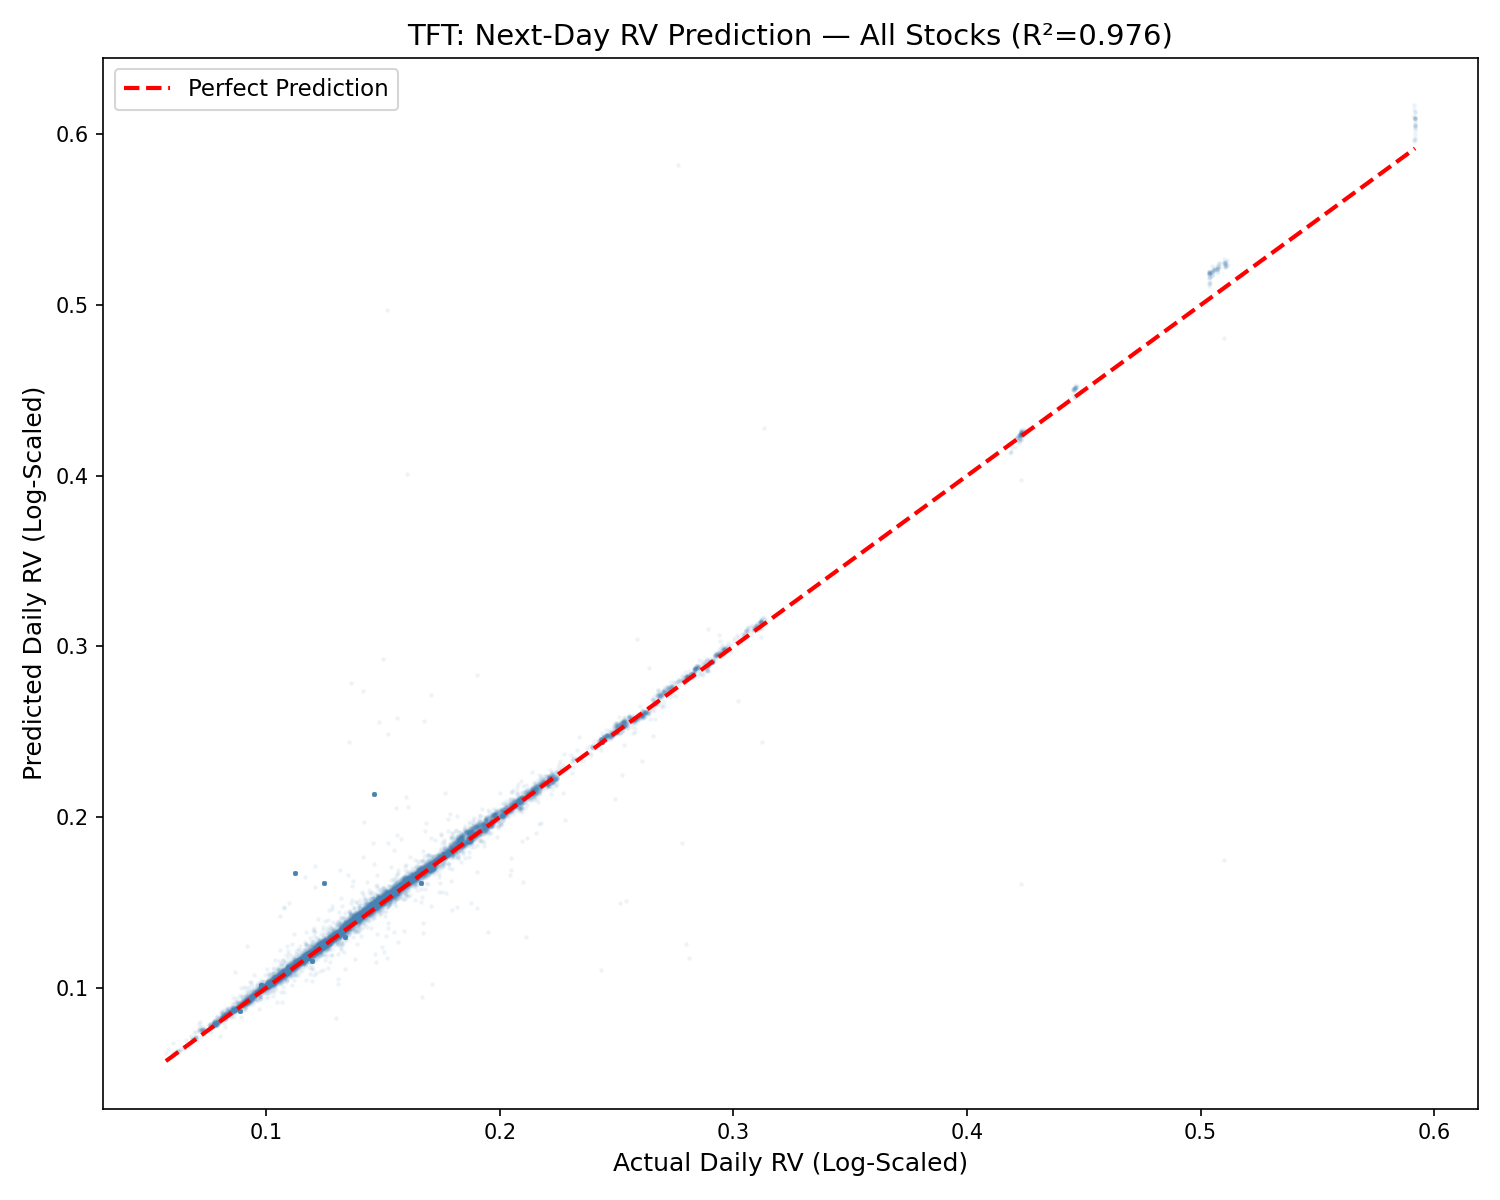
\includegraphics[width=0.80\textwidth]{Figures/scatter_pred_vs_actual_daily.png}
\caption{Model~A predictions versus actual observation.}
\label{fig:scatter}
\end{figure}

\section{Discussions}

\subsection{Interpretability: Variable Selection Network}

One of the main selling points of the TFT is that you can actually look inside it and see what it is doing. Figure~\ref{fig:importance} shows the encoder-side feature importance weights produced by the VSN. The one-day lagged realised volatility (\texttt{RV\_1d\_lag75}) receives a weight of 60.4, absolutely dwarfing everything else by two orders of magnitude. This is not just a nice number---it means the TFT has independently rediscovered the HAR-RV structure from data alone. The daily lag dominates for the same reason that $\beta_d$ dominates in the classical regression: daily persistence is the single strongest signal in the data.

\begin{figure}[!t]
\centering
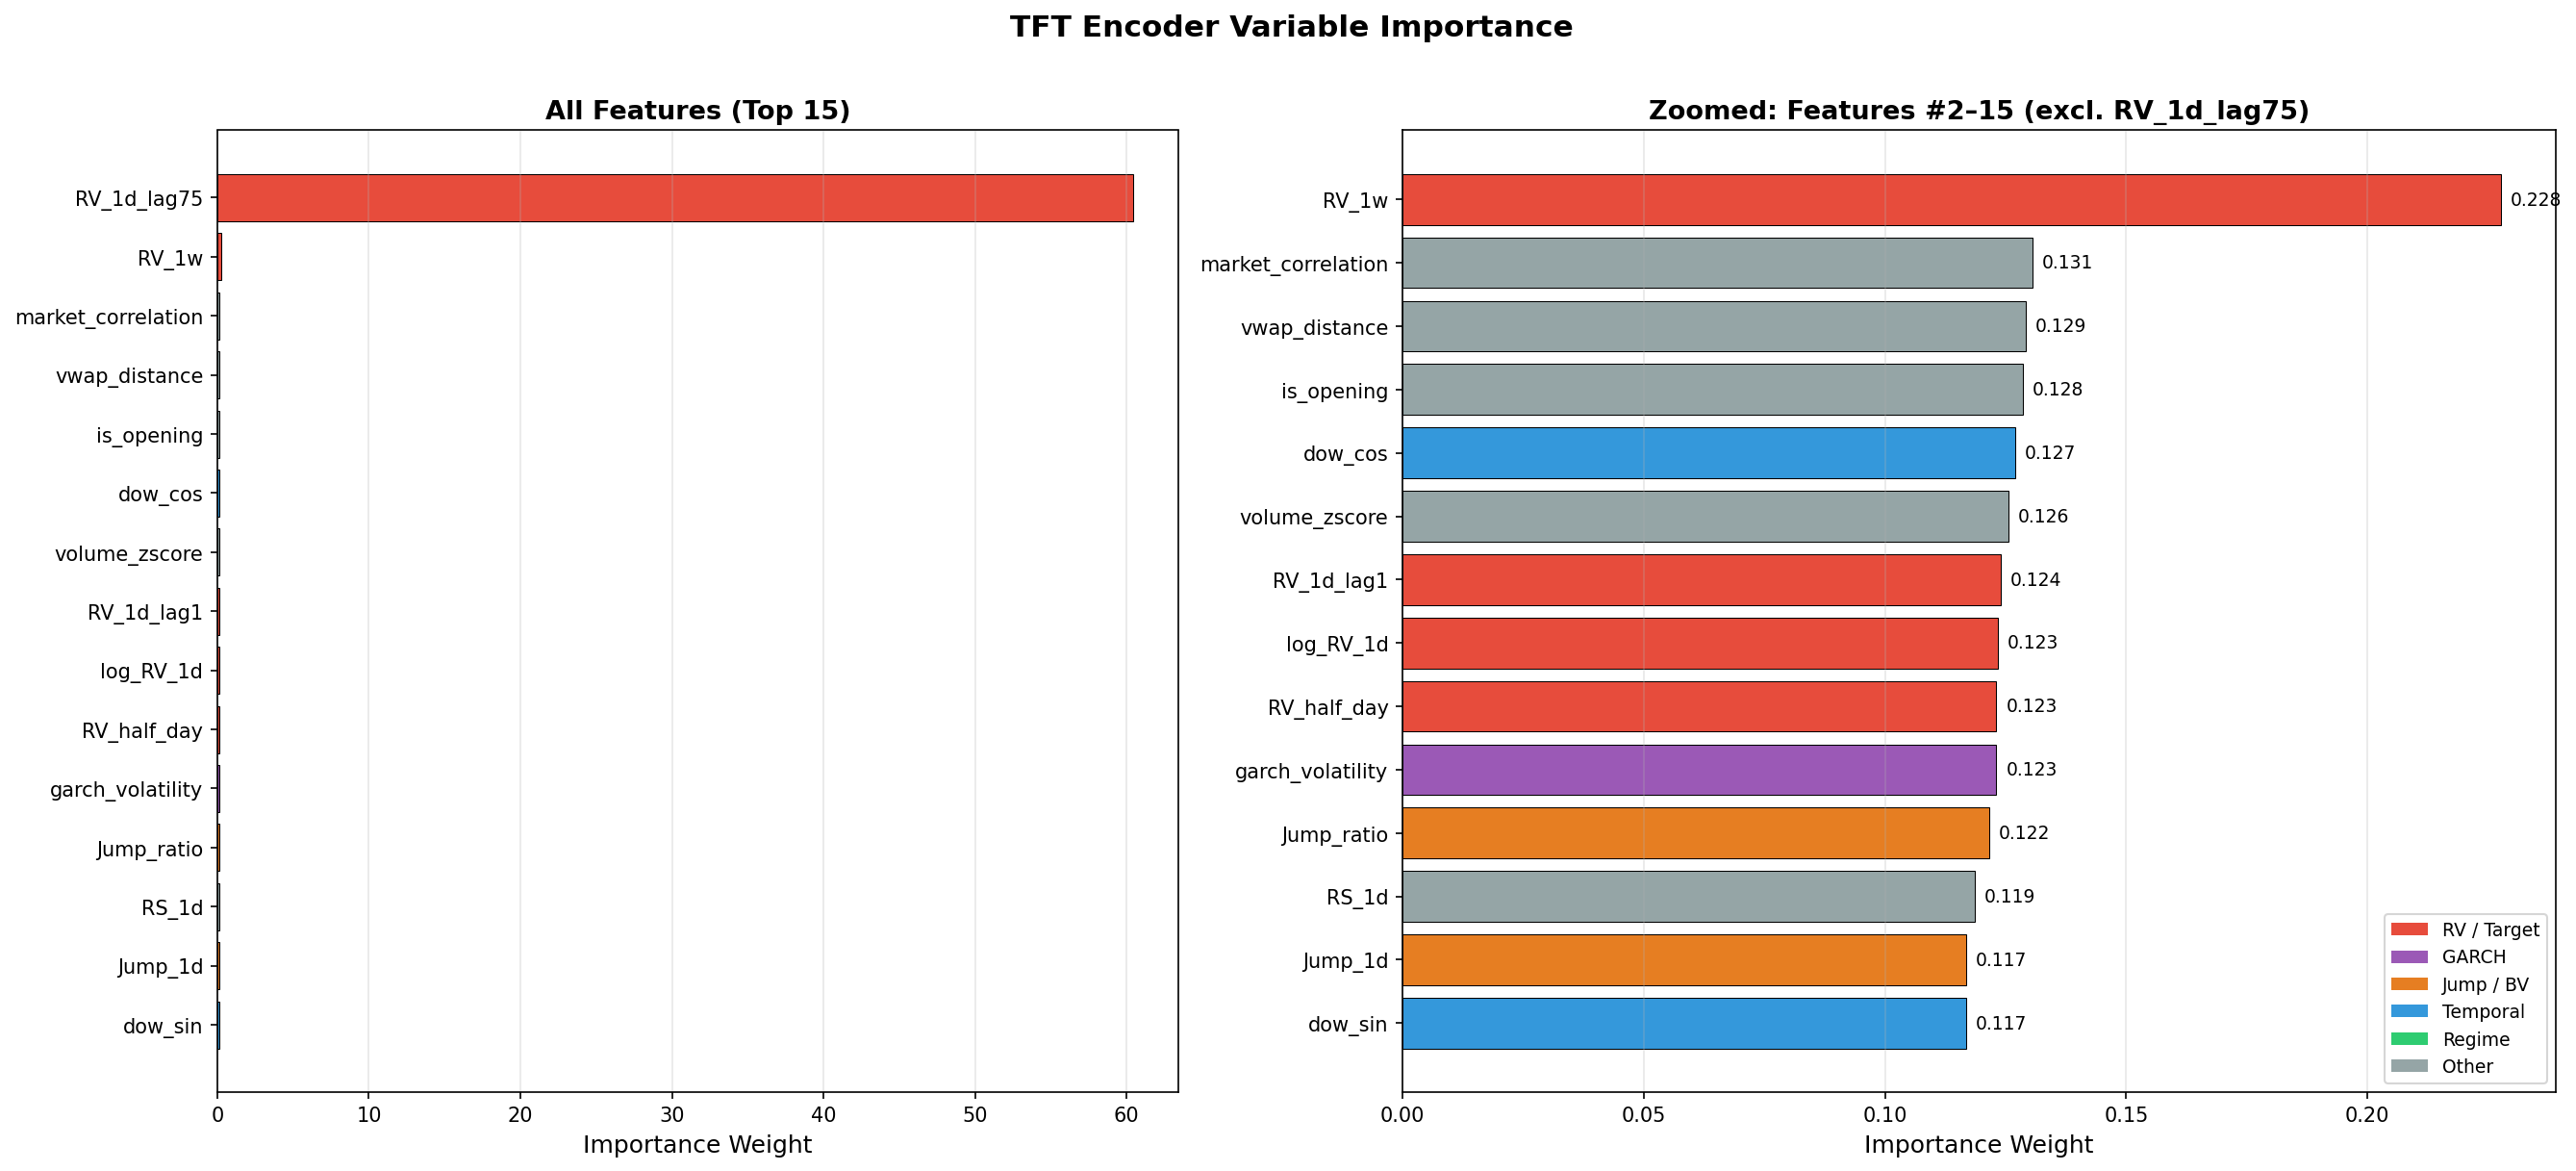
\includegraphics[width=\textwidth]{Figures/variable_importance.png}
\caption{Variable Selection Network encoder importance weights. RV\_1d\_lag75 dominates at 60.4.}
\label{fig:importance}
\end{figure}

The secondary features are interesting in their own right: weekly RV gets a weight of 0.23, market correlation gets 0.13, and GARCH conditional variance gets 0.12. On the decoder side, \texttt{is\_opening} receives the highest weight (32.3), which aligns perfectly with the elevated price-discovery volatility in the first 15 minutes of the Indian session.

\subsection{Data Integrity}

We took three specific precautions to ensure the results are trustworthy. First, every feature uses data at or before bar $t$, while the target uses bars $t+1$ through $t+75$---zero temporal overlap, no leakage. Second, the train-validation split is strictly chronological with no shuffling whatsoever. Third, the 98.7\% bar overlap between consecutive daily targets is a structural property of the rolling RV estimator, not a data handling error. The ablation study explicitly controls for this overlap by comparing models with and without the lagged target, so any inflation due to persistence is isolated and measured rather than ignored.



\section{Project Impact and SDG Compliance}

\textbf{Environmental.} Training used $\sim$120 GPU hours on Kaggle's free T4 tier, consuming roughly 14.4~kWh and emitting about 5.8~kg~CO$_2$e. Inference runs on CPU at under 1~W per prediction. \textbf{(SDG~12: Responsible Consumption.)}

\textbf{Societal.} Better volatility forecasts help retail investors size positions sensibly, allow fund managers to shift allocations dynamically, and give regulators better market-stability monitoring tools. The TFT's built-in interpretability makes the framework auditable---critical for regulated deployment. All code and preprocessing scripts are documented and publicly available, serving as ready-made material for graduate courses in financial ML. \textbf{(SDG~4: Quality Education; SDG~8: Decent Work.)}

\textbf{Innovation.} The RA-TFT combines decades of econometric intuition (GARCH, HAR-RV, HMM) with a modern Transformer, producing a hybrid that is genuinely novel. The entire project ran on free infrastructure, lowering the barrier for smaller firms and academic groups. \textbf{(SDG~9: Industry and Innovation.)}

\section{Conclusions}

\begin{enumerate}
\item We collected, cleaned, and enriched $\sim$2.65 million five-minute bars across fourteen NSE stocks, engineering 47 features spanning six established categories.
\item The RA-TFT achieved $R^2 = 0.976$ and MAPE = 1.90\%, within one percentage point of HAR-RV ($R^2 = 0.983$), while offering cross-stock generalisation and full VSN interpretability.
\item The ablation separated persistence ($\sim$72~pp of explained variance) from genuine feature-driven prediction ($R^2 = 0.258$), confirming that engineered features carry real but modest signal.
\item Regime-conditioned evaluation revealed best performance in the High Volatility regime ($R^2 = 0.999$) and worst in Extreme ($R^2 = 0.765$), pinpointing tail forecasting as the key improvement area.
\item The VSN independently rediscovered the HAR-RV lag structure, assigning weight 60.4 to the daily lag---a striking data-driven validation of classical econometric insight.
\end{enumerate}

\section{Scope for Future Work}

Six directions merit exploration: (1)~regime-specific ensembles gated by HMM state; (2)~exogenous features such as RBI text embeddings and options-implied volatility; (3)~multi-horizon (weekly/monthly) forecasting; (4)~formal Diebold-Mariano testing for pairwise statistical significance; (5)~live REST API deployment with real-time NSE ingestion and scheduled retraining; (6)~cross-market generalisation to other emerging markets.
